\documentclass[rapport.tex]{subfiles}

\begin{document}
	\subsection{Analyse descendante}
		\begin{center}
			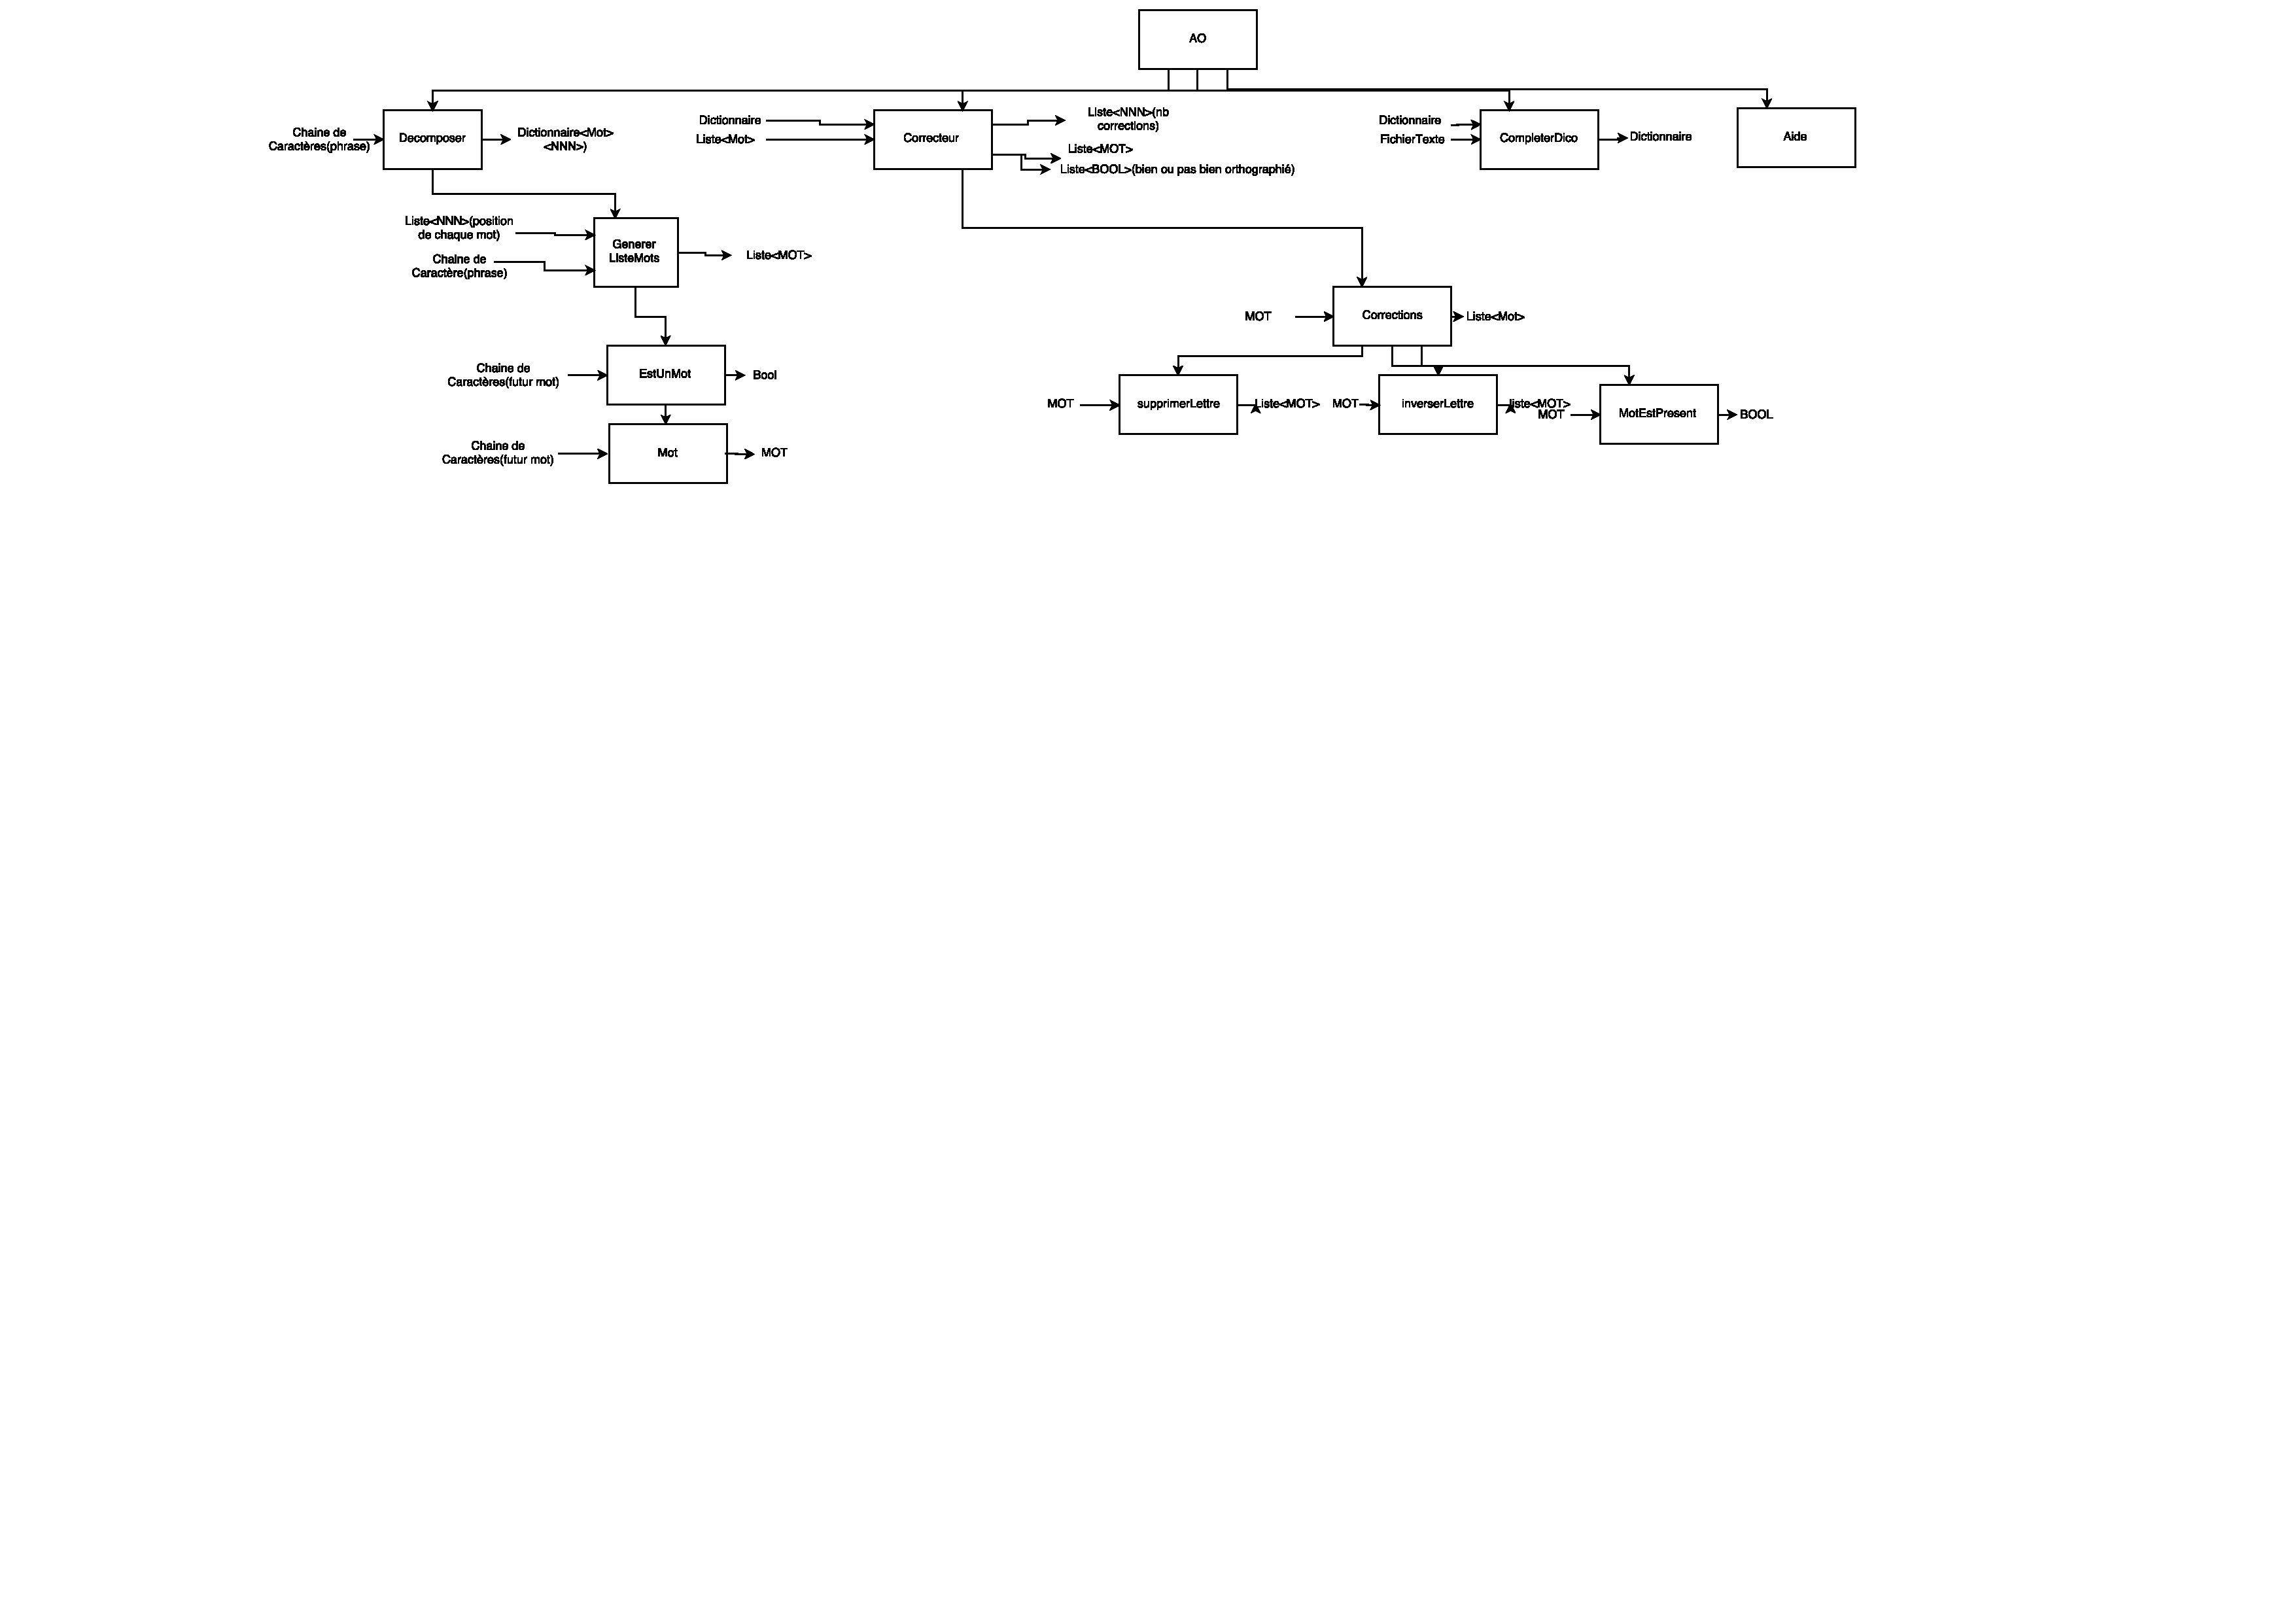
\includegraphics[width=20cm,angle=-90]{images/AnalyseDescendante}
		\end{center}
		
	\subsection{TAD Mot}
	
	\begin{tad}
		\tadNom{Mot}
		\tadDependances{\caractere, \chaine, \naturelNonNul, \booleen}
		\begin{tadOperations}{supprimerLettre}			
			\tadOperation{estUnMot}{\tadUnParam{\chaine}}{\tadUnParam{\booleen}}
			
			\tadOperationAvecPreconditions{mot}{\tadUnParam{\chaine}}{\tadUnParam{\textbf{Mot}}}

			\tadOperation{longueurMot}{\tadUnParam{Mot}}{\tadUnParam{\naturelNonNul}}
			
			\tadOperationAvecPreconditions{iemeCaractere}{\tadDeuxParams{Mot}{\naturelNonNul}}{\tadUnParam{\caractere}}	

			\tadOperation{supprimerLettre}{\tadUnParam{Mot}}{\tadUnParam{Tableau de \textbf{Mot}}}
			
			\tadOperation{inverserLettre}{\tadUnParam{Mot}}{\tadUnParam{Tableau de \textbf{Mot}}}
			
		    \tadOperation{motEnChaine}{\tadUnParam{Mot}}{\tadUnParam{\chaine}}	
				
		\end{tadOperations}     
	
		\begin{tadSemantiques}{}
		\tadSemantique{estUnMot}{vérifie si un mot est bien une chaine composée uniquement de lettres}
		\tadSemantique{mot}{transforme une chaine de caractères en un Mot}
		\tadSemantique{supprimerLettre}{génère un tableau contenant toutes les combinaisons possibles de suppression d'une lettre du Mot}
		\tadSemantique{inverserLettre}{génère un tableau contenant toutes les combinaisons possibles d'inversion de deux lettres consécutives du Mot}
		\tadSemantique{motEnChaine}{transforme un Mot en une chaine de caractères}
		
		\end{tadSemantiques}
		
		\begin{tadPreconditions}{}
			\tadPrecondition{mot(chaine)}{estUnMot(chaine)}					
			\tadPrecondition{iemeCaractere(chaine,i)}{1 $\leq$ i $\leq$ longueur(chaine)}			
			
		\end{tadPreconditions}
	\end{tad}
	
	\newpage
	\subsection{TAD Dictionnaire}
	
	\begin{tad}
		\tadNom{Dictionnaire}
		\tadParametres{}
		\tadDependances{fichierTexte, Mot, \booleen, \naturel}
		\begin{tadOperations}{creationDictionnaire}
			
			\tadOperation{DICTIONNAIRE_completerDico}{\tadDeuxParams{Dictionnaire}{FichierTexte}}{\tadUnParam{Dictionnaire}}
			
			
			\tadOperation{DICTIONNAIRE_motDansDico}{\tadDeuxParams{Dictionnaire}{Chaîne de caractères}}{\tadUnParam{\booleen}}
		
			\tadOperationAvecPreconditions{DICTIONNAIRE_ajouterDico}{\tadDeuxParams{Dictionnaire}{Chaîne de caractères}}{\tadUnParam{Dictionnaire}}

			\tadOperationAvecPreconditions{DICTIONNAIRE_detruireDico}{\tadUnParam{Dictionnaire}{Dictionnaire}{Mot}}{\tadUnParam{Dictionnaire}}			
			
		\end{tadOperations}
		
		\begin{tadAxiomes}
			
		\end{tadAxiomes}
	
		\begin{tadSemantiques}{chercherMot}
		\tadSemantique{motEstPresent}{Indique si le mot est present dans le dictionnaire}
			
		\end{tadSemantiques}
		
		\begin{tadPreconditions}{insererNouveauMot}
			\tadPrecondition{insererNouveauMot}{non(motEstPresent(dico,mot))}
			\tadPrecondition{supprimerMot}{motEstPresent(dico,mot)}
			
			
			
		\end{tadPreconditions}
	\end{tad}
	
	\newpage
	\subsection{TAD CorrecteurOrthographique}
	
	
	\begin{tad}
		\tadNom{CorrecteurOrthographique}
		\tadParametres{}
		\tadDependances{Dictionnaire, Mot, \booleen, \naturel}
		\begin{tadOperations}{correcteurOrthographique}
			
			\tadOperation{correcteurOrthographique}{\tadUnParam{Dictionnaire}}{\tadUnParam{CorrecteurOrthographique}}
			
			\tadOperation{corriger}{\tadDeuxParams{Dictionnaire}{Mot}}{\tadUnParam{Liste de mots}}
			
			\tadOperationAvecPreconditions{decomposer}{\tadUnParam{\chaine}}{\tadUnParam{Liste de mots}}
			
			\tadOperation{nbMots}{\tadUnParam{\chaine}}{\tadUnParam{\naturel}}
			
			\tadOperation{estCorrigeable}{\tadUnParam{\chaine}}{\tadUnParam{\booleen}}
		\end{tadOperations}
		
		\begin{tadAxiomes}
			
		\end{tadAxiomes}
	
		\begin{tadSemantiques}{}
			\tadSemantique{corriger}{Permet de générer une liste de mots corrigés possibles appartenant au dictionnaire après la génération de mots aléatoires}
			\tadSemantique{decomposer}{Génère une décomposition de la chaîne en une liste de mots contenant chaque mot de la chaîne entrée}
		\end{tadSemantiques}
	
		\begin{tadPreconditions}{}
			\tadPrecondition{corriger}{non(estVide(\chaine))}
		\end{tadPreconditions}
	\end{tad}
\end{document}
